\chapter{Spanner}
\label{chapter:spanner}

Given a graph \(G\) with a genus of at most \(g\), a set of pairs of terminals \(\mathcal{D}\), and a constant \(\epsilon > 0\), we aim to generate a subgraph \(H\) of \(G\) with the following properties. 

\begin{itemize}
    \item Quasi-optimality Property: There is a collection of cycles in \(H\) that connects all pairs of terminals in \(\mathcal{D}\) and has a maximum length of \((1 + c \epsilon) \opt_{\mathcal{D}}(G)\) (with \(c\) constant), in particular \(\opt_{\mathcal{D}}(H) \leq (1 + c \epsilon) \opt_{\mathcal{D}}(G)\);
    \item Shortness Property: The total length of \(H\) is at most \(f(\epsilon, g) \cdot \opt_{\mathcal{D}}(G)\), where \(f(\epsilon, g)\) is a constant dependent on \(\epsilon\) and the genus \(g\) of \(G\).
\end{itemize}

It is worth mentioning that the Quasi-optimatily property is also know in the literature as Spanning property.

We formalize the concept of a \textbf{spanner} graph with the following Theorem.

\begin{theorem}\label{theorem:spanner}
Given \(\epsilon > 0\) fixed, a bounded-\textit{genus} graph \(G_{in} = (V_{in}, E_{in})\) and a set of pairs of terminals \(\mathcal{D}\), we can calculate in polynomial-time a spanner \(H\) of \(G_{in}\) for Steiner Multicycle with respect to \(\mathcal{D}\).
\end{theorem}

To build a spanner \(H\), we need to apply the PC-Partition technique introduced in Chapter~\ref{chapter:pc-partition}. This technique returns a set of components that will serve as the basis for constructing a new structure called \textit{Mortar Graph}.

Throughout this chapter, for each component \(C_i\) obtained from Theorem~\ref{theoremClustering}, consider \(T_i\) as a spanning tree of \(C_i\).

\section{Mortar Graph}

The \textit{Mortar Graph} was proposed in \cite{Borradaile2009b} for planar graphs and was later expanded in \cite{Borradaile2012} for bounded-genus graphs.

It is a grid-like subgraph that spans all terminals and has size \(\mathcal{O}(\opt)\). Each face of the Mortar Graph contains a subgraph named \textbf{brick}. The crossing between a brick and the rest of the graph can only be done through a limited set of vertices called \textbf{portals}, which bounds the number of possible solutions.

The Mortar Graph is built for each \(T_i\) obtained from the clustering step (Chapter~\ref{chapter:pc-partition}) individually to create a subgraph \(H_i\) of \(G\).

\subsection{Cut graph construction}

Given a graph \(G\) of genus \(g\) embedded in a surface of same genus and a connected subgraph \(H\) of \(G\) we define the process of \textbf{cutting} \(G\) with \(H\) by duplicating every edge of \(H\), along with the vertices, and creating a new face in the embedding of the graph inside the duplicated edges of \(H\). This process is illustrated in Figure~\ref{fig:cut_graph_example}.

\begin{figure}[h]
    \centering
    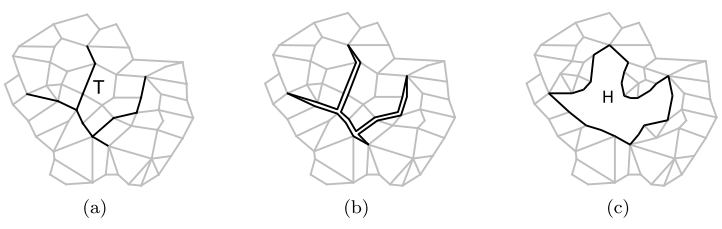
\includegraphics[scale=0.7]{imgs/cut_graph_example.png}
    \caption {Example of cutting process using a subgraph \(T\) to form a face \(H\) inside the graph. (\cite{Borradaile2012}).}
    \label{fig:cut_graph_example}
\end{figure}

% It is worth mentioning that if the subgraph used to do the cutting has cycles, the cutting process may disconnect components of the original graph.

From that, we define a \textbf{cut graph} \(CG\) as a subgraph of \(G\) that when used to cut \(G\) results in a planar graph.

The goal of this section is to find a \textbf{cut graph} \(CG\) of \(G\) that contains all terminals and whose length is bounded by a constant times \(\opt\). Cutting \(G\) using \(CG\) results in a planar graph with a cycle \(\sigma\) as the boundary, where \(\sigma\) is twice the length of \(CG\).

Figure~\ref{fig:mortar5} illustrates the process of cutting a graph of genus greater than 0.  Figure~\ref{fig:mortar5}(a) shows a cut graph drawn on a torus, while Figure~\ref{fig:mortar5}(b) shows the result of cutting the surface along the graph: the shaded area is homeomorphic to a disk, and the light area is the additional face of the planarized surface.

\begin{figure}[h]
    \centering
    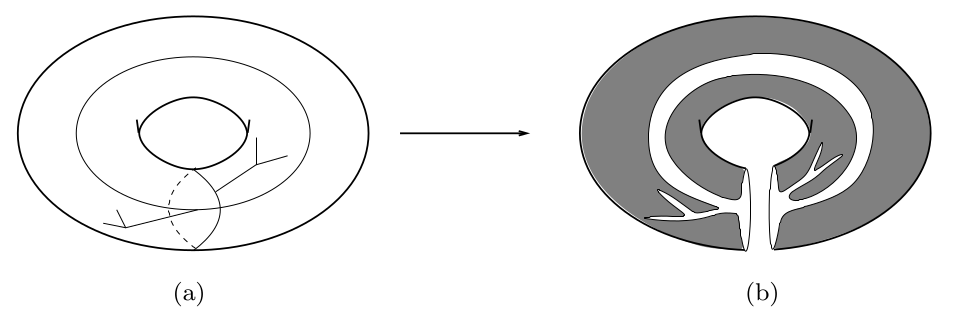
\includegraphics[scale=0.45]{imgs/mortar5.png}
    \caption {Example of a cut in a graph with \textit{genus} greater than zero. (\cite{Borradaile2012}).}
    \label{fig:mortar5}
\end{figure}


\cite{Borradaile2012} observed that, given a planar graph \(G\) and a spanning tree \(T\) of \(G\). Then the set of edges \(E(G) - E(T)\) induces a spanning tree \(T^{\star}\) in the dual graph \(G^{\star}\). Furthermore, if \(T\) is a minimal spanning tree of \(G\), then \(T^{\star}\) is a maximal spanning tree of \(G^{\star}\). This result was derived by \citeauthor{Borradaile2012} from the Lemma~1 of \cite{EPPSTEIN199233}.

The result can be generalized for bounded \textit{genus} graphs: If \(T\) is a minimum spanning tree of \(G\) and \(T^{\star}\) the maximum spanning tree of \(G^{\star} - E(T)\), then \(T^{\star}\) is a maximum spanning tree of \(G^{\star}\) and the size of the set of remaining edges \(X := E(G) - E(T) - E(T^{\star})\) is \(g\), or the Eulerian \textit{genus} of \(G\), obtained by Euler's formula. \cite{Eppstein} define such a triple \((T, T^{\star}, X)\) as the \textit{tree-cotree decomposition} of \(G\), and shows that a cut graph can be generated from the decomposition.

\begin{figure}[H]
    \centering
\begin{tikzpicture}


    \Vertex[x=0, y=2, color=white, Math,IdAsLabel]{A}
    \Vertex[color=white, Math,IdAsLabel]{B}

    \Vertex[x=1, y=1, color=white, Math,IdAsLabel]{C}
    \Vertex[x=2, y=0, color=white, Math,IdAsLabel]{D}

    \Vertex[x=1, y=-0.3, color=white, Math,IdAsLabel]{E}
    \Vertex[x=2, y=1.5, color=white, Math,IdAsLabel]{F}

    \Vertex[x=3, y=0, color=white, Math,IdAsLabel]{G}
    \Vertex[x=3, y=1.5, color=white, Math,IdAsLabel]{H}

    \Edge[opacity=1.0](A)(B)
    \Edge[opacity=0.3](A)(F)
    \Edge[opacity=1.0](A)(C)
    \Edge[opacity=1.0](C)(F)
    
    \Edge[opacity=0.3](A)(E)
    \Edge[opacity=1.0](C)(E)
    \Edge[opacity=0.3](D)(E)

    

    
    \Edge[opacity=0.3](F)(H)
    \Edge[opacity=0.3](H)(G)
    \Edge[opacity=0.3](G)(D)
    \Edge[opacity=0.3](D)(F)
    \Edge[opacity=0.3](F)(G)
    \Edge[color=green](D)(H)

    \Edge[color=red](F)(H)
    \Edge[color=red](F)(D)
    

\end{tikzpicture}
    \caption{Example of \(loop(T, e)\). The tree \(T\) is rooted at the vertex \(F\) and is represented by the black (non-opaque) edges. The edge \(e\) of the loop is represented in green and the paths between \(e\) and the vertex \(F\) are displayed in red. The \(loop(T, e)\) is composed of the union of the red and green edges.}
    \label{fig:loop_T_e}
\end{figure}


Let \(T\) be a spanning tree rooted at a vertex \(r\), and let \(e\) be an edge not contained in \(T\). We say that \(loop(T, e)\) is the simple cycle formed by \(e\) and the paths between \(r\) and both ends of \(e\) (exemplified in Figure~\ref{fig:loop_T_e}). Based on the results from \citeauthor{Eppstein}, \cite{Borradaile2012} showed:

\begin{lemma}[\cite{Borradaile2012}, Lemma 1]
    Given a tree-cotree decomposition \((T, T^{\star}, X)\), \(\{loop(T, e): e \in X\}\), is a cut graph.
\end{lemma}

The construction of the cut graph follows from \cite{Borradaile2012}, with slight technical changes. We start with \(T_i\) (which is a minimum spanning tree of the component \(C_i\) calculated in Algorithm~\ref{algorithm:pc-partition}) and contract it to a vertex \(r\).

We then find a shortest-path tree \(SPT\) rooted at \(r\), uncontract \(r\) back into \(T_i\) and set \(T := T_i \cup SPT\), where \(T\) is a spanning tree of \(G\). With that, we can then find a spanning tree \(T^\ast\) of \(G^\ast - E(T)\) using the results presented above.

Let \(X := E(G) - E(T) - E(T^\ast)\). As the output cut graph we return \(CG := T_i \cup \{loop(T, e): e \in X\}\).

We proceed to cut \(G\) using \(CG\) and duplicate each edge and vertex of \(CG\). Thus, generating a cycle \(\sigma\) internal to the clipping of \(CG\). After this process, let \(G_1\) be the planar graph obtained from \(G\). Finally, we invert the face \(\sigma\) in such a way that \(\sigma\) becomes the new external face of \(G_1\). From construction and Theorem~\ref{theoremClustering}, \(\ell(\sigma)\) is at most \(c \cdot \opt\) where \(c\) is a constant.

\citeauthor{Borradaile2012} refers to the algorithm presented above as \textbf{Planarize algorithm} and formalizes the result with the Lemma:

\begin{lemma}[\cite{Borradaile2012}, Lemma 2]
    The algorithm \textbf{Planarize} returns a cut graph \(CG\) such that cutting \(G\) open along \(CG\) results in a planar graph \(G_p\) with face \(f_\sigma\) whose facial walk \(\sigma\)

    \begin{enumerate}
        \item is a simple cycle,
        \item contains all terminals (some terminals might appear more than once as multiple copies might be created during the cutting process); and
        \item has length \(\ell(\sigma) \leq c \opt\) for \(c > 0\) constant.
    \end{enumerate}
\end{lemma}

\subsection{Strips}

To continue with the algorithm, we need to present the following definition. Given $\epsilon > 0$ and a graph \(G\), a path \(P\) in \(G\) is \(\epsilon\)-\textit{short} if in each pair of vertices \((x, y) \in P\) the distance between \(x\) and \(y\) in \(P\) is at most \((1 + \epsilon)\) times the distance \(x\) and \(y\) in \(G\), in other words, \(dist_P(x, y) \leq (1 + \epsilon) dist_G(x, y)\).

We proceed to decompose the planar graph \(G_1\) into \textit{strips}. Let \(\sigma[x, y]\) be the path between \(x\) and \(y\) in \(\sigma\) in the counterclockwise direction of the \textit{planar embedding} of \(G_1\) into a sphere. If \(x = y\), by convention \(\sigma[x, y] = \sigma\).

In order to segment \(G_1\) into strips, we find vertices \(x\) and \(y\) in \(\sigma\) such that \(\sigma[x, y]\) is the shortest path of \(\sigma\) which is not \(\epsilon\)-\textit{short} in \(\sigma\). Such a pair of vertices always exists since \(\sigma[x, y]\), with \(x = y\), is not \(\epsilon\)-\textit{short}. Let \(N\) be the shortest path between \(x\) and \(y\) in \(G_1\). Certainly \(\ell(N) < \ell(\sigma[x, y])\). We call \textbf{strip} the subgraph covered by \(N \cup \sigma[x, y]\). This process is performed recursively on the subgraph of \(G_1\) covered by \(N \cup (\sigma - \sigma[x, y])\). As a result, we have \(G_1\) segmented by strips. Items~(a) and (b) of Figure~\ref{fig:mortar2} illustrate this process.

\begin{figure}[h]
    \centering
    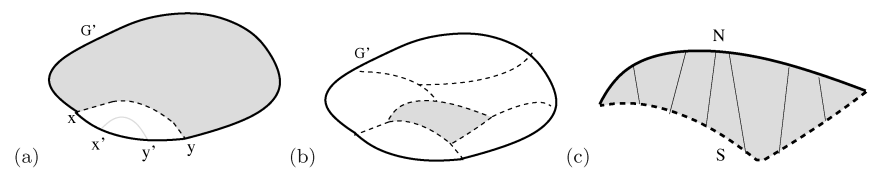
\includegraphics[scale=0.5]{imgs/mortar2.png}
    \caption{Construction of strips in Mortar Graph (\cite{Borradaile2009b}).}
    \label{fig:mortar2}
\end{figure}

In Figure~\ref{fig:mortar2}, Item~(a) shows the first track is created by a path (dashed) connecting \(x\) and \(y\). The distance between every pair of vertices \(x'\) and \(y'\), between \(x\) and \(y\) on the boundary, is well approximated by the distance on the boundary. We use recursion in the shaded area; Item~(b) shows how a graph is divided into bands (by the dashed lines). A strip is increased in Item~(c). Columns (vertical lines) are taken from the set of shortest paths between the ``low'', or south boundary (dashed line) and the ``up'', or north boundary (solid line).

\begin{lemma}[\cite{klein2006}, inequality (10)] \label{strip_length}
The total length of the boundary of all strips is at most \((\frac{1}{\epsilon} + 1)\) times the length of \(\sigma\).
\end{lemma}

\citeauthor{klein2006} also showed that the strip decomposition of a planar graph with \(n\) vertices can be found in \(\mathcal{O}(n \log n)\).

Given a fixed strip, we denote \(N\) as the north-boundary of the strip and \(S\) as the south-boundary.

With the graph \(G_1\) decomposed into strips, as illustrated in Item~(b) of Figure~\ref{fig:mortar2}. The next step is, for each strip, to calculate the shortest paths, called \textit{columns}. Consider a strip with north and south boundaries, \(N\) and \(S\) respectively. We select vertices \(s_0, s_1, \dots\) in \(S\) as follows. We embed the north strip above the south strip, directing \(S\) and \(N\) from left to right. Let \(s_0\) be the leftmost vertex common to \(S\) and \(N\). By convention, the column \(C_0\) is defined as the shortest path between \(s_0\) and \(N\), in this case, an empty path.

For \(i \geq 1\), find the first vertex in \(S\) (from left to right) such that the length of the path from \(s_{i-1}\) to \(s_i\) in \(S\) is greater than \(\epsilon\) times the length of the shortest path from \(s_i\) to \(N\) within the strip. That is, \(dist_S(s_{i-1}, s_i) > \epsilon \cdot dist_{strip}(s_i, N)\). Thus, column \(C_i\) is defined as the shortest path between \(s_i\) and \(N\) in the strip, as illustrated by Item~(c) of Figure~\ref{fig:mortar2}.

\begin{lemma}[\cite{klein2006}, Lemma 5.2]
The sum of all column lengths in a strip is at most \(\epsilon^{-1} \cdot \ell(S)\).
\end{lemma}

After having the columns calculated, for each strip, we have a set \(C_0, C_1, \dots, C_s\) of columns of the strip.

For \(\epsilon > 0\), let \(\kappa = \kappa(\epsilon) = 4 \epsilon ^ {-2} (1 + \epsilon ^ {-1})\). We will use this constant on the following definition and for the following lemmas due to \cite{Borradaile2009b}.

% Let \(\mathcal{C}_i = C_i \cup C_{i+\kappa} \cup C_{i+2\kappa} \cup \dots\) for \(i \in \{0, 1, \dots, \kappa - 1\}\).
Let \(\mathcal{C}_i = \bigcup_{j=0}^{\kappa-1} C_{i+j\kappa}\) for \(i \in \{0, 1, \dots, \kappa - 1\}\).

Let \(i^\ast\) be the index that minimizes \(\ell(\mathcal{C}_i)\). We designate the columns of \(\mathcal{C}_i^\ast\) as \textbf{super-columns}.

\begin{lemma}[\cite{Borradaile2009b}, Lemma 6.5]
The sum of the lengths of the supercolumns in a strip is at most \(\kappa^{-1}\) times the sum of the lengths of the columns in the strip.
\end{lemma}

\begin{lemma}[\cite{Borradaile2009b}, Lemma 6.6] \label{borradaile_2009b_lemma_6_6}
     The sum of the lengths of all the supercolumns over all strips is at most \(c \epsilon \opt\), where \(\epsilon > 0\) and \(c > 0\) depends on \(\epsilon\).
\end{lemma}

We define as the \textbf{Mortar Graph} \(MG\) of \(G\) the embedded planar subgraph generated by the edges of \(T_i\), the edges of the strips, and the edges of super-columns.

\begin{figure}[h]
    \centering
    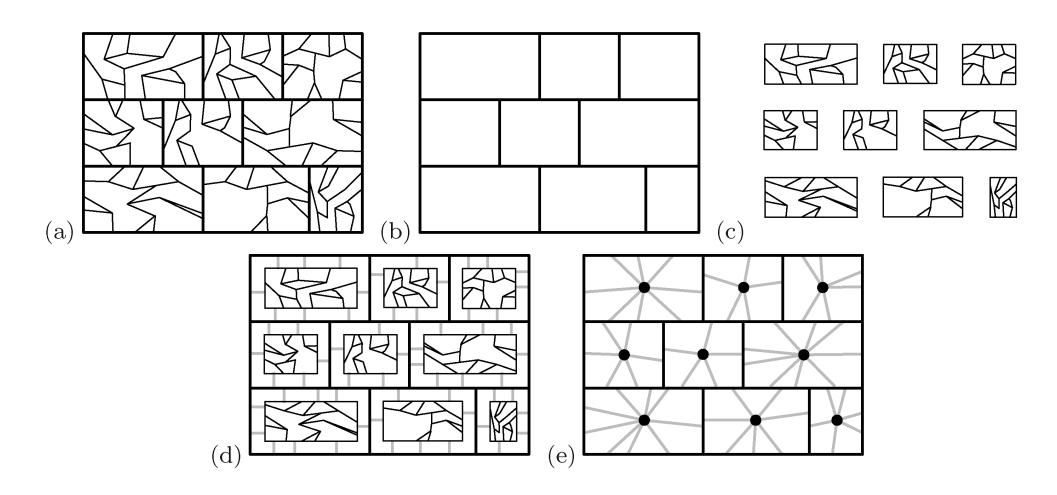
\includegraphics[scale=0.4]{imgs/mortar3.png}
    \caption{Mortar Graph. (\cite{Borradaile2009b}).}
    \label{fig:mortar3}
\end{figure}

Item~(a) shows the graph \(G_1\), highlighting the edges of the Mortar Graph. 
Item~(b) shows only the Mortar Graph \(MG\) obtained. 
Item~(c) shows the set of bricks corresponding to \(MG\). 
Item~(d) illustrates a portal-connected graph \(\mathcal{B}^{+}(MG)\) (will be presented ahead), where the portal edges are gray. 
Item~(e) shows \(\mathcal{\mathcal{B}}^{+}(MG)\) with the bricks contracted into vertices, resulting in \(\mathcal{B}^{\div}(\mathcal{B }^{+}(MG))\).

We note two properties derived from the results presented during the construction of \(MG\). First, let \(Q\) be the set of all terminals of \(G\), by construction, we have that \(Q \subseteq V(MG)\). The second property is presented below.

\begin{lemma} \label{length_mg}
     \(\ell(MG) \leq c \epsilon \sigma\) with \(c > 0\) constant.
\end{lemma}
\begin{proof}
    The result follows from Theorem~\ref{theoremClustering} and Lemmas~\ref{strip_length} and~\ref{borradaile_2009b_lemma_6_6}.
\end{proof}

\subsection{Bricks}

To create a \textbf{brick} (illustrated in  Figure~\ref{fig:mortar3}(c)), for each face \(f\) of \(MG\), we duplicate the border edges and vertices of \(f\). This results in a disconnected induced subgraph of \(G_1\) that is entirely contained within the ``external'' copy of \(f\)'s border (Figure~\ref{fig:mortar4}(c)). The result of this process can be seen in Figure~\ref{fig:mortar4}.

Figure~\ref{fig:mortar4}(a) illustrates the boundary of a face \(f\) of \(MG\) as a cycle of edges (thick edges), possibly with repetition (that is, an edge can occur twice at the border). The light edges are those inside \(f\) in \(G\). Figure~\ref{fig:mortar4}(b) shows an example of brick \(B\) obtained by the process described above. \(B\) has boundary \(\partial B\). Figure~\ref{fig:mortar4}(c) shows a brick \(B\) contained within the ``external'' copy of the border of \(f\).

\begin{figure}[h]
    \centering
    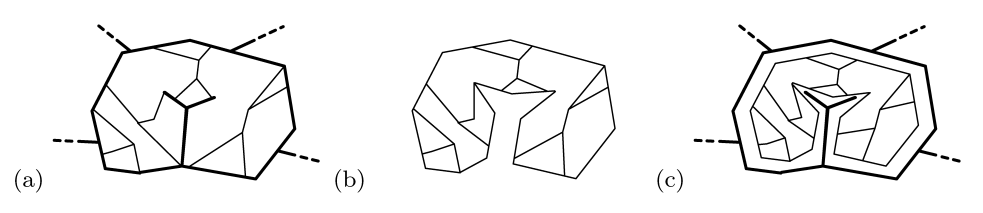
\includegraphics[scale=0.45]{imgs/mortar4.png}
    \caption{Construction of a brick. (\cite{Borradaile2009b}).}
    \label{fig:mortar4}
\end{figure}

The boundary \(\partial B\) of a brick \(B\) is the simple cycle formed by the edges of the boundary. The corresponding face of \(MG\) is called \textbf{mortar boundary} from~\(B\). Each edge of \(MG\) occurs at most in the disjoint union of the boundary of the bricks.

\begin{lemma}[\cite{Borradaile2009b}, Lemma 6.10]
    A mortar boundary \(B\), in counterclockwise order, is the concatenation of four paths \(W\), \(S\), \(E\), \(N\) (west, south, east, north) such that:
    \begin{enumerate}
        \item The set of edges \(B - \partial B\) is nonempty.
        \item Every vertex of \(\mathcal{D} \cap B\) is in \(N\) or in \(S\).
        \item \(N\) is \(0\)-short in \(B\), and every proper subpath of \(S\) is \(\epsilon\)-short in S.
        \item There exist \(k \leq \kappa\) vertices \(s_0, s_1, s_2, \dots, s_k\) ordered from west to east along \(S\) such that, for any vertex \(x\) of \(S[s_i, s_{i+1})\), the distance from \(x\) to \(s_i\) along \(S\) is less than \(\epsilon\) times the distance from \(x\) to \(N\) in \(B\), that is, \(dist_S(x, s_i) < \epsilon dist_B(x, N)\).
    \end{enumerate}
\end{lemma}

\subsection{Portals}

The connection between a face \(f\) of \(MG\) and its respective brick \(B\) is performed through a subset of vertices of \(\partial B\) called \textbf{portals}. This connection is made in such a way that, for each portal \(p\) of \(\partial B\), an edge with weight 0 is placed between \(p\) and the vertex of which it was duplicated in \(\partial f\).

For each brick \(B\), we set some vertices of \(\partial B\) as \textbf{portals}. We define \(\theta = \theta(\epsilon) = 18 \cdot \alpha(\epsilon) \cdot \epsilon ^ {-2}\). Where \(\alpha(\epsilon)\) is a constant that will be defined later.

For portal selection, we use the following greedy algorithm. An initial vertex \(v_0\) of \(\partial B\) is selected with uniform probability. Then we define \(v_1\) as the first vertex of \(\partial B\) clockwise such that \(\ell(\partial B[v_0, v_1]) > \ell(\partial B) / \theta\). This process is repeated for \(v_i\) in \(\partial B\) until \(v_0 \in V(\partial B (v_{i-1}, v_i))\).

Using the previous construction, we get the following properties given by \cite{Borradaile2009b}.

\begin{lemma}[\cite{Borradaile2009b}, Lemma 7.1] \label{lemma:cobertura}
(Cover property): For any vertex \(x \in \partial B\), there exists a portal \(y\) such that the \(x\)-to-\(y\)-subpath of \(\partial B\) has a maximum length \(\ell(\partial B) / \theta\).
\end{lemma}

\begin{lemma}[\cite{Borradaile2009b}, Lemma 7.2]
(Cardinality property): There are at most \(\theta\) portals in \(\partial B\).
\end{lemma}

With that, we have a Mortar Graph \(MG\) with a set of bricks connected with the face boundaries of \(MG\) through portal edges, as illustrated by Item~(d) Figure~\ref{fig:mortar3}. This construction is named by \citeauthor{Borradaile2009b} as portal-connected graph, and is represented as \(\mathcal{B}^{+}(MG)\).

\section{Spanner construction}

Finally, we proceed to prove Theorem~\ref{theorem:spanner}.

We start by building a separate subgraph \(H_i\) for each \(T_i\). Initially, \(H_i\) is a Mortar Graph created from \(T_i\). Following that, for each brick \(B\) and a selection of its portals \(\Pi' \subseteq \Pi\), we add to \(H_i\) an optimal Steiner Tree that reaches \(\Pi'\) and uses only edges from the interior of \(B\) or its boundary. This can be done in polynomial time in \(\theta\) using the algorithm proposed in \cite{ericksonST}, since all terminals lie on the infinite face of a planar graph.

Note that for fixed \(\epsilon\) and \(g\) there is at most a constant number of portals, hence a constant number of such Steiner Trees, and the length of each is at most the length of the boundary of the brick \(B\).

We will leverage an auxiliary result to prove both spanner properties.

\begin{lemma}\label{lemma:borradaile_10_1}
    Let \(G\) be a planar embedded graph and let \(C\) be a subgraph of \(G\) that intersects a \(\epsilon\)-short path \(P\). There is a subpath of \(P\) spanning the vertices of \(C \cap P\) whose total length is \((1 + \epsilon) \ell(C)\)
\end{lemma}
\begin{proof}
    Let \(P'\) be the shortest subpath of \(P\) that spans all the vertices of \(C \cap P\). There is a path \(Q\) in \(C\) that connects all vertices of \(C \cap P\). Since \(P\) is \(\epsilon\)-short \(\ell(P') \leq (1 + \epsilon)\ell(Q) \leq (1 + \epsilon)\ell(C)\)
\end{proof}

\begin{lemma} [\cite{Bateni}, Lemma 4.1] \label{bateni_4_1_forest}
    For any forest \(F\) in a brick \(B\), there exists a forest \(F'\) such that
\begin{enumerate}
    \item \(\ell(F') \leq (1 + \epsilon)\ell(F)\)
    \item \(F'\) crosses the boundary of \(B\) at most \(\alpha\) times
    \item any two vertices on \(N-\) or \(S-\)boundaries of \(B\) connected by \(F\) are also connected by \(F'\)
\end{enumerate}
\end{lemma}

In Corollary~\ref{bateni_4_1_multicycle}, we will generalize the result above to a collection of cycles (instead of a forest), but first, we need to introduce the concept of \textbf{cleaving}.

Put simply, cleaving is the process of breaking a vertex into two new vertices and adding an artificial, zero-cost edge between them. It can be formalized as: given a vertex \(v\) and a bipartition \(A, B\) of the edges incident to \(v\), split \(v\) into two new vertices \(v_A\) and \(v_B\). Then, connect the endpoints of the edges in \(A\), previously connected to \(v\), to \(v_A\), and the edges in \(B\) to \(v_B\). Finally, add a zero-cost edge \(e_{AB}\) between \(v_A\) and \(v_B\). This operation is illustrated in Figure~\ref{fig:cleaving} (a) and (b).

There can be two types of cleaving:
\begin{itemize}
    \item Simplifying Cleaving (Figure~\ref{fig:cleaving} (c) and (d)). Let \(C\) be a clockwise, non-self-crossing (i.e., planar) non-simple cycle that visits a vertex \(v\) twice. Defined a bipartition of the edges incident to \(v\) as follows: given the clockwise embedding of the edges incident to \(v\), let \(A\) start and end with consecutive edges of \(C\) and contain only two edges of \(C\), let \(B\) be the remaining edges. Such a bipartition exists because \(C\) is non-self-crossing.
    \item Lengthening Cleaving (Figure~\ref{fig:cleaving} (e) and (f)). Let \(C\) be a simple cycle, and let \(v\) be a vertex on \(C\) with two edges \(e_A\) and \(e_B\) adjacent to \(v\) embedded strictly inside \(C\), and let \(e'_A\) and \(e'_B\) be consecutive edges of \(C\) adjacent to \(v\) such that the following bipartition is non-crossing concerning the embedding: \(A\), \(B\) is a bipartition of the edges adjacent to \(v\) such that \(e_A, e'_A \in A\) and \(e_B, e'_B \in B\).
\end{itemize}

\begin{figure}[h]
    \centering
    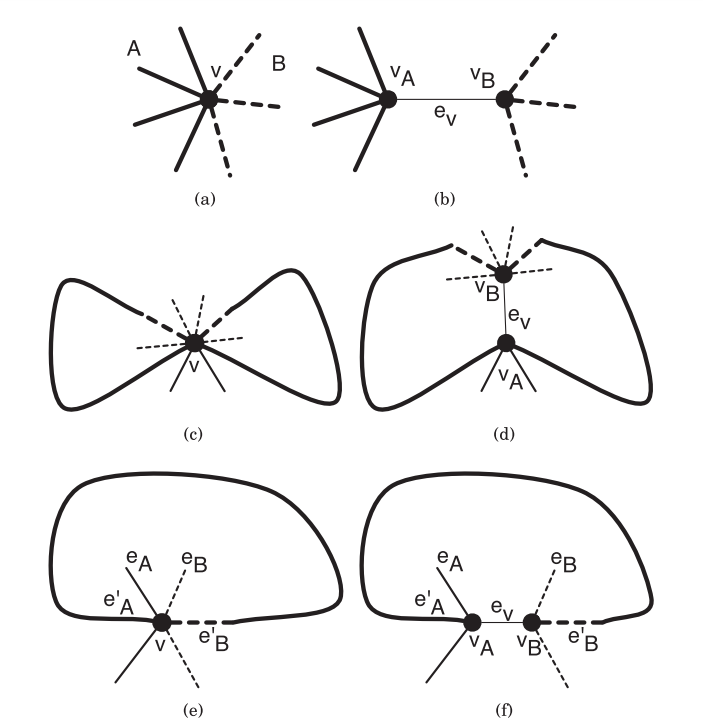
\includegraphics[scale=0.5]{imgs/cleaving.png}
    \caption{Cleavings illustrated (\cite{borradaile_2EC}).}
    \label{fig:cleaving}
\end{figure}

\begin{corollary}\label{bateni_4_1_multicycle}
For any collection of cycles \(M\) in a brick \(B\), there is a collection of cycles \(M'\) such that
\begin{enumerate}
    \item \(\ell(M') \leq (1 + c \epsilon)\ell(M)\)
    \item \(M'\) crosses the boundary of \(B\) at most an \(\alpha\) (constant) number of times
    \item any two vertices on \(N-\) or \(S-\)boundaries of \(B\) connected by \(M\) are also connected by \(M'\)
\end{enumerate}
\end{corollary}
\begin{proof}
    Let \(M^\ast\) be an optimal solution to the SMCP in \(G\) and let \(MG\) be a Mortar Graph built from \(G\). 

    For a given brick \(B\) (with \(W, N, E, S\) boundaries), let \(M\) be the intersection between \(M^\ast\) and \(B\). Note that \(M\) might be composed of cycles and trees (e.g., cycle fragments that connect to themselves outside the brick) and each vertex in \(M \cap \partial B\).

    We begin the construction of \(M_1\) by adding the \(W\) and \(E\) boundaries of \(B\) to \(M\). We know from Lemma~\ref{borradaile_2009b_lemma_6_6} that the cost of the union of \(M^\ast\) with all super-columns (i.e., the west and east boundaries of all bricks) is at most \((1 + 2 c \epsilon) \opt\).

    To streamline the rest of the proof, we perform the simplifying cleaving on non-simple cycles of \(M_1\) until all cycles become simple (also accounting for duplicated edges).
    We can have two situations for each component \(C\) of \(M_1\):
    \begin{enumerate}
        \item \(C\) connects vertices in \(N\) or vertices in \(S\)
        \item \(C\) connects vertices from \(N\) and \(S\)
    \end{enumerate}

    To tackle case (1), we use Lemma~\ref{lemma:borradaile_10_1} to replace the path of \(C\) that connects two vertices in \(N\) with a subpath of \(N\), which connects the same vertices. Since \(N\) is a \(\epsilon\)-path, the Lemma holds, and the increase in cost is limited by a \((1 + \epsilon)\) factor.

    For case (2), we apply the lengthening cleaving to the boundary of brick \(B\). For each vertex \(v\) in \(M_1 \cap \partial B\) that has a degree greater than one, we perform the lengthening cleaving in \(v\). We repeat this process while there are still multiple edges of the solution embedded in a brick that is incident to a shared boundary vertex. In other words, we have that the intersection of \(M_1\) with the interior of brick \(B\) is a subgraph whose joining vertices with \(\partial B\) have degree one.


    The first property follows, since - as mentioned - in case (1), the increase in cost is limited by a \((1 + \epsilon)\) factor, and in case (2) we only add zero-cost edges.
    
    To get the second and third properties, we can directly apply Lemma~\ref{bateni_4_1_forest} (Structural properties of Bricks) on \(M_1\). 
\end{proof}

Considering the final spanner \(H\) to be the union of all \(H_i\)'s, we proceed to prove that \(H\) indeed respects both properties of \textbf{quasi-optimality} and \textbf{shortness}.

\begin{lemma}{{(Shortness property).}}\label{spanner_shortness_property} Given a graph \(G\) and a subgraph \(H\) of \(G\) constructed with the process above, the length of \(H\) is at most \(f(\epsilon, g) \opt\) for a certain function
\(f(\epsilon, g)\).
\end{lemma}
\begin{proof}
Note that each \(H_i\) is constructed from \(MG_i\) (which by its turn is built from \(T_i\)), a set of portal edges connected to \(MG_i\), and a limited set of Steiner Trees inside the bricks. By Lemma~\ref{length_mg}, \(\ell(MG_i) \leq f(\epsilon, g) \ell(T_i)\). For each brick \(B\), we add at most \(2^{\theta}\) trees, each with length no more than \(\ell(\partial B)\). Since each edge of \(MG_i\) may appear in at most two bricks, the total length is bounded by \(2^{\theta + 1} \ell(MG_i)\). Therefore, \(\ell(H_i) \leq 2^{\theta + 1} \ell(MG_i) = f(\epsilon, g) \ell(T_i)\).

By Theorem~\ref{theoremClustering}, the sum of the length of all \(T_i\) is no more than \((16/\epsilon + 4) \opt_{\mathcal{D}}(G_{in})\).
This implies that the sum of the length of all \(H_i\) is no more than \(f(\epsilon, g) (16/\epsilon + 4) \opt_{\mathcal{D}}(G_{in})\).
\end{proof}

\begin{lemma}\label{spanner_quasi_optimality_property}
    Quasi-optimality property.~\(\opt_{\mathcal{D}}(H) \leq (1 + c \epsilon) \opt_{\mathcal{D}}(G_{in})\) with \(c\) and \(\epsilon\) constants.
\end{lemma}
\begin{proof}

    Let \(\{C_i\}_{i=1}^k\) be the set of components outputted by Algorithm~\ref{algorithm:pc-partition}.

    From Theorem~\ref{theoremClustering}, we have that \(\sum_{i}^k \opt_{\mathcal{D}_i} \leq (1 + \epsilon) \opt_{\mathcal{D}}\). So we can focus on proving that \(\opt_{\mathcal{D}_i}(H_i) \leq (1 + c \epsilon) \opt_{\mathcal{D}_i}(G_{in})\).

    Consider each \(H_i\) as formed in the process above, so each \(H_i\) is formed by a Mortar Graph built using \(T_i\) (a minimum spanning tree of \(C_i\) from Theorem~\ref{theoremClustering}), the portal edges and the set of Steiner Trees connecting the portals in each Brick.

    Let \(M^\ast_i\) be an optimal solution for the SMCP considering \(\mathcal{D}_i\), i.e. \(\ell(M^\ast_i) = \opt_{\mathcal{D}_i}(G_{in})\). We add the set of all supercolumns in \(H_i\) to \(M^\ast_i\) to get \(M^1_i\). Recall that, by Lemma~\ref{borradaile_2009b_lemma_6_6}, the length of these supercolumns is at most \(c \epsilon \opt_{\mathcal{D}_i}(G_{in})\).

    Next, we replace the intersection of \(M_i^1\) and each brick with another subgraph having the properties of  Corollary~\ref{bateni_4_1_multicycle}. Let \(M_i^2\) be the new subgraph. The length of the solution increases to no more than a \(1 + c \epsilon\) factor.

    From  Corollary~\ref{bateni_4_1_multicycle}, we know that \(M_i^2\) crosses each brick at most \(\alpha\) times, so we can ensure that moving these intersection points to the portals adds no more than a constant factor in the length.

    Consider a brick \(B\) with boundaries \(W, N, E, S\). Connect each intersection point of the brick to its closest portal. Each connection on a brick \(B\) moves by at most \(2 \ell(\partial B) / \theta\). Therefore, the total movement of each brick is at most \(\alpha 2 \ell(\partial B) / \theta\), which is no more than \(2 \epsilon^2 \ell(\partial B) / \gamma(\epsilon, g)\). Hence, the total additional length for all bricks of \(H_i\) is bounded by \(4 \epsilon^2 \ell(T_i)\). Let \(M_i^3\) be the resulting subgraph.

    Hence the length of \(M_i^3\) is at most \(4 \epsilon^2 \ell(T_i) + \ell(M_i^2)\). Considering that \(\ell(M_i^2) \leq (1 + \epsilon) \ell(M_i^1)\) and \(\ell(M_i^1) \leq \epsilon^2 \ell(T_i) + M^\ast_i\), we have that \(\ell(M_i^3) \leq 4 \epsilon^2 \ell(T_i) + (1 + \epsilon) \ell(M^\ast_i)  + \epsilon^2 \ell(T_i)\)

    Let \(M' = \bigcup_i^k M_i^3\). Accounting that \(\sum_i^k \ell(T_i) \leq (4/\epsilon + 4) \opt\) (from Theorem~\ref{theoremClustering}), it holds that \[\ell(M') \leq \sum_i^k \left ( 4 \epsilon^2 \ell(T_i) + (1 + \epsilon) \ell(M^\ast_i)  + \epsilon^2 \ell(T_i) \right).\] 
    Therefore, we can conclude that  \(\ell(M') \leq (1 + 21 \epsilon + 20 \epsilon^2) \opt = (1 + c'\epsilon) \opt\).
\end{proof}
